% Packages used
\documentclass{article}
\usepackage[letterpaper, portrait, margin=2cm]{geometry}
\usepackage[utf8]{inputenc}
\usepackage[spanish, mexico]{babel}
\usepackage[T1]{fontenc}
\usepackage{float}
\usepackage{url}
\usepackage{hyperref}
\hypersetup{
    colorlinks=true,
    linkcolor=blue,
    filecolor=magenta,      
    urlcolor=cyan,
    pdftitle={Escornabot Brivoi Compactus},
    pdfpagemode=FullScreen,
}
\usepackage{array}
\usepackage{longtable}
\usepackage{multirow}
\renewcommand{\arraystretch}{1.2}
\usepackage{siunitx}
\usepackage{booktabs}
\usepackage{makecell}
\usepackage[table,xcdraw]{xcolor}
\usepackage{graphicx}
\graphicspath{ {./images/Botonera/} }
\usepackage{gensymb}
\usepackage{caption}
\usepackage{subcaption}
\captionsetup[sub]{
    labelfont = bf,
    margin = 12pt,
%    indention = 18pt,
} 


%Beginning of the document
\title{Manual de Ensamble Robot Escornabot Brivoi Compactus}
\author{Wilmer Gaona Romero (@wgaonar)}
\date{Julio 2020}

\begin{document}

\maketitle

\begin{figure}[H]
    \centering
    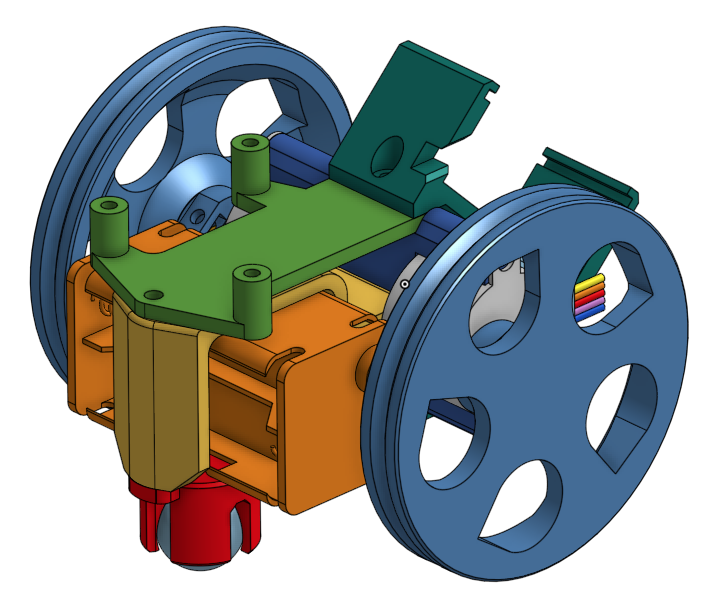
\includegraphics[width=0.5\columnwidth]{images/portadaOnshape.png}
    \caption{Modelo 3D del Escronabot Brivoi Compactus}
    \label{fig:modelo3D}
\end{figure}

\section{Introducción}
Escornabot es un robot móvil de software y hardware abierto diseñado para la enseñanza de electrónica y programación en niños, adolescentes y no tan niños. Basado en la tarjeta Arduino Nano, destaca la sencillez de su diseño mecánico, electrónico y la estructura del código con el cual funciona. Todo esto ha sido posible por la comunidad que lo desarrolla y mantiene actualizado. Existen diversas versiones y la que corresponde a este manual es la \textbf{Brivoi Compactus} la cual utiliza dos tarjetas de circuitos impresos (PCB):

\begin{enumerate}
     \item Tarjeta de la botonera: \href{https://github.com/xdesig/escornabot-electronics/tree/master/Electronics/E_KEYPAD/E_KEYPAD_2.20}{E\_KeyPad V2.2 diseñada por XDeSIG}
     \item Tarjeta de control basada en el Arduino Nano:
     \href{https://github.com/xdesig/escornabot-electronics/tree/master/Electronics/EscornaCPU/1.x/1.20}{EscornaCPU V1.2 diseñada por XDeSIG}
\end{enumerate}

\subsection{Lista de Componentes Electrónicos}
La Tabla \ref{tab:componentes_general} detalla la cantidad, descripción y la tarjeta en la que irán colocados (Botonera o la CPU) cada uno de los componentes del Escornabot. 

\begin{longtable}{|c|m{0.4\textwidth}|c|c|}
    \caption{Lista de Componentes para el Escornabot} \label{tab:componentes_general} \\ \hline 
    \multicolumn{1}{|c|}{\cellcolor[HTML]{C0C0C0}\textbf{\makecell{CANTIDAD \\ TOTAL}}} &
    \multicolumn{1}{c}{\cellcolor[HTML]{C0C0C0}\textbf{DESCRIPCIÓN}} & 
    \multicolumn{1}{|c|}{\cellcolor[HTML]{C0C0C0}\textbf{\makecell{CANTIDAD \\ BOTONERA}}} & \multicolumn{1}{c|}{\cellcolor[HTML]{C0C0C0}\textbf{\makecell{CANTIDAD \\ CPU}}} \\ \hline 
    \endfirsthead
    \caption{Lista de Componentes para el Escornabot - Continuación} \\ \hline
    \multicolumn{1}{|c|}{\cellcolor[HTML]{C0C0C0}\textbf{\makecell{CANTIDAD \\ TOTAL}}} &
    \multicolumn{1}{|c|}{\cellcolor[HTML]{C0C0C0}\textbf{DESCRIPCIÓN}} & 
    \multicolumn{1}{c|}{\cellcolor[HTML]{C0C0C0}\textbf{\makecell{CANTIDAD \\ BOTONERA}}} & \multicolumn{1}{c|}{\cellcolor[HTML]{C0C0C0}\textbf{\makecell{CANTIDAD \\ CPU}}} \\ \hline
    \endhead
    1 & Tarjeta EscornaCPU versión 1.2 & - & 1 \\ \hline
    1 & Tarjeta E\_KeyPad versión 2.2 & 1 & - \\ \hline
    1 & Arduino Nano & - & 1 \\ \hline
    2 & Motor paso a paso 28BYJ-48 & - & 2 \\ \hline
    1 & Driver ULN2803 & - & 1 \\ \hline
    1 & Zócalo de 18 pines para el driver ULN2803 & - & 1 \\ \hline
    1 & Portapilas para 4 pilas AA & - & -  \\ \hline
    1 & Terminal T-block de 5mm para alimentación & - & 1 \\ \hline
    4 & Resistencia 1 K$\Omega$ & 4 & - \\ \hline
    9 & Resistencia 10 K$\Omega$ & 5 & 4\\ \hline
    1 & Resistencia 18 K$\Omega$ o de 20K$\Omega$ & - & 1 \\ \hline
    1 & Resistencia 22 K$\Omega$ o de 20K$\Omega$ & 1 & -\\ \hline
    1 & Led de 3mm Azul & 1 & - \\ \hline
    1 & Led de 3mm Rojo &  1 & - \\ \hline
    1 & Led de 3mm Amarillo&  1 & - \\ \hline
    1 & Led de 3mm Verde &  1 & -\\ \hline
    5 & Pulsadores de 12mm &  5 & -\\ \hline
    7 & Pines/headers macho a 90\degree & 7 & - \\ \hline
    8 & Pines/headers macho rectos  & - & 8 \\ \hline
    1 & Puente o Jumper para pines rectos  & - & 1 \\ \hline
    2 & Tira de 15 pines hembra que serán la base sobre la cual se colocará el Arduino Nano & - & 2 \\ \hline
    1 & Tira de 4 pines hembra si posteriormente se desea conectar un adaptador Bluetooth para conectar el robot con una aplicación para teléfono móvil. & - & 1 \\ \hline
    1 & Interruptor de alimentación SK12D07 & - & 1 \\ \hline
    2 & Conector macho para motor paso a paso JST-XHP-S & - & 1 \\ \hline
    1 & Buzzer pasivo para Arduino & - & 1 \\ \hline
    1 & Fusible rearmable XF050 & - & 1 \\ \hline
    1 & Diodo Schottky 1N5817 & - & 1 \\ \hline
    2 & Condensadores cerámicos 104 de 100nF & - & 2 \\ \hline
    6 & Cables Dupont hembra - hembra de 10cm & 6 & - \\ \hline
\end{longtable}

A continuación se detalla el proceso de ensamble de las partes, componentes y tarjetas de circuito impreso.

\section{Ensamble y soldadura de la tarjeta de la botonera E\_KeyPad versión 2.2}

\subsection{Lista de componentes de la Botonera}
La Tabla \ref{tab:componentes_botonera} muestra a detalle la cantidad de los componentes, la etiqueta en la tarjeta y la función que desempeñan.

\begin{longtable}{|c|>{\raggedright}m{0.2\textwidth}|>{\centering}m{0.15\textwidth}|m{0.45\textwidth}|}
    \caption{Descripción y funcionamiento de los componentes requeridos para la botonera} \label{tab:componentes_botonera} \\ \hline 
    \multicolumn{1}{|c|}{\cellcolor[HTML]{C0C0C0}\textbf{CANT.}} &
    \multicolumn{1}{c}{\cellcolor[HTML]{C0C0C0}\textbf{DESCRIPCIÓN}} & 
    \multicolumn{1}{|c|}{\cellcolor[HTML]{C0C0C0}\textbf{ETIQUETA}} & \multicolumn{1}{c|}{\cellcolor[HTML]{C0C0C0}\textbf{FUNCIÓN}} \\ \hline 
    \endfirsthead
    \caption{Componentes requeridos para la botonera - Continuación} \\ \hline
    \multicolumn{1}{|c|}{\cellcolor[HTML]{C0C0C0}\textbf{\makecell{CANT.}}} &
    \multicolumn{1}{c}{\cellcolor[HTML]{C0C0C0}\textbf{DESCRIPCIÓN}} & 
    \multicolumn{1}{|c|}{\cellcolor[HTML]{C0C0C0}\textbf{ETIQUETA}} & \multicolumn{1}{c|}{\cellcolor[HTML]{C0C0C0}\textbf{FUNCIÓN}} \\ \hline 
    \endhead
    4 & Resistencia 1 K$\Omega$ & R6, R8, R9, R10 & Resistencia para la activación de los Leds de la botonera. \\ \hline
        \multirow{2}{*}{5} 
        & \multirow{2}{*}{Resistencia 10 K$\Omega$} & R1, R2, R3, R4  & Conforman el divisor de voltaje en conjunto con los botones para obtener diferentes valores de acuerdo al botón o switch que se ha presionado y así controlar el movimiento deseado:
        \begin{itemize}
            \item El botón S1 conectado con R1 selecciona un movimiento hacia ADELANTE.
            \item El botón S2 conectado con R2 selecciona un giro hacia la IZQUIERDA.
            \item El botón S3 conectado con R3 selecciona un movimiento hacia ATRÁS.
            \item El botón S5 conectado con R4 ejecuta la secuencia de movimientos introducida, es decir, es el botón: GO.
        \end{itemize} \\ \cline{3-4}
        &  & R7 & \textcolor{red}{Opcional:} Está presente en la botonera en caso de que se utilice una tarjeta de control diferente a la EscornaCPU V1.2 y en la que no se utilice la resistencia interna de PULL-UP del Arduino Nano. En el firmware del robot se tendría que definir la palabra clave: KEYBOARD\_WIRES con el valor de 3. Por precaución, esta resistencia se puede soldar. \\ \hline
        1 & Resistencia 22 K$\Omega$ o de 20 K$\Omega$ & R5 & La última resistencia  del divisor de voltaje: 
        \begin{itemize}
            \item El botón S4 conectado con R5 selecciona un giro hacia la DERECHA.
        \end{itemize}\\ \hline
        1 & Led de 3mm Azul & LED1 & Led indicador de un movimiento hacia ADELANTE. \\ \hline
        1 & Led de 3mm Rojo & LED2 & Led indicador de un movimiento hacia IZQUIERDA. \\ \hline
        1 & Led de 3mm Amarillo & LED3 & Led indicador de un movimiento hacia ATRÁS. \\ \hline
        1 & Led de 3mm Verde & LED4 & Led indicador de un movimiento hacia DERECHA. \\ \hline
        \multirow{2}{*}{5}
        & \multirow{2}{*}{Pulsadores de 12mm} & S1, S2, S3, S4 & Botones para elegir los movimientos a realizar (ADELANTE, IZQUIERDA, ATRÁS Y DERECHA).\\ \cline{3-4}
        & & S5 & Botón GO que ejecuta la secuencia de los movimientos elegidos.\\ \hline 
\end{longtable}

\subsection{Soldadura de las Resistencias}
Las resistencias no tienen polaridad, así que no importa la orientación en que sean colocadas. Para proceder a soldarlas, colocar las resistencias teniendo presente que los valores correspondan con las etiquetas en la tarjeta. Las Figuras \ref{fig:botonera_resistencias_parte1} y \ref{fig:botonera_resistencias_parte2} muestra los pasos para soldar las resistencias. Tener cuidado con la ubicación de R5 para evitar confundirla con las demás ya que solo se utiliza una. (ver Figura \ref{fig:botonera_resistencias5}) .

\begin{figure}[htbp]
    \centering
    \begin{subfigure}[t]{0.3\textwidth}
        \centering
        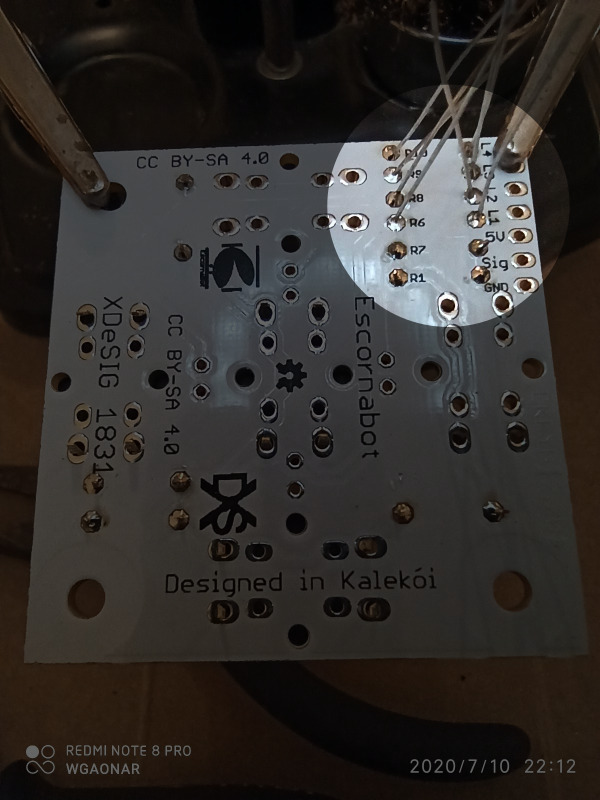
\includegraphics[width=0.9\columnwidth, height=1.2\columnwidth]{images/Botonera/botonera1.jpg}
        \caption{PCB de la botonera vista por debajo con resistencias colocadas para soldar.}
        \label{fig:botonera_resistencias1}
    \end{subfigure}%
    \begin{subfigure}[t]{0.3\textwidth}
        \centering
        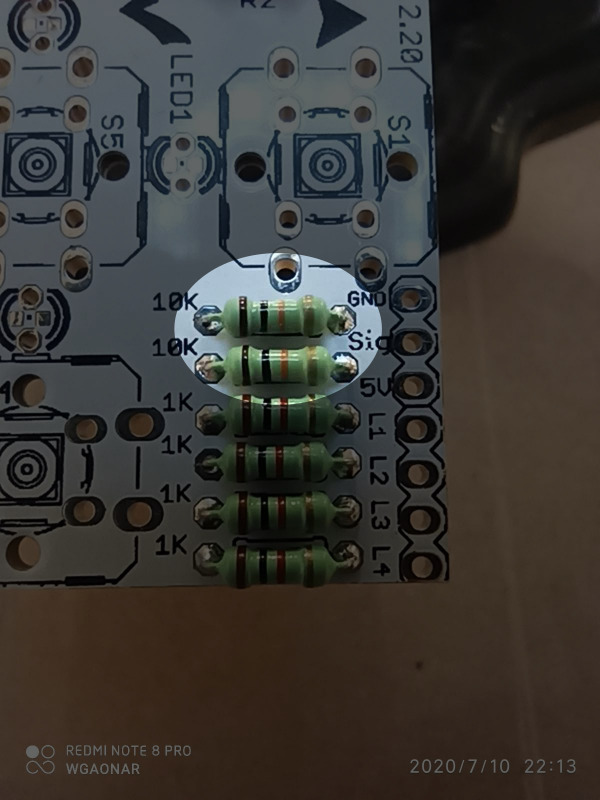
\includegraphics[width=0.9\columnwidth, height=1.2\columnwidth]{images/Botonera/botonera2.jpg}
        \caption{Resistencias R1 y R7 de 10 K$\Omega$}
        \label{fig:botonera_resistencias2}
    \end{subfigure}%
    \begin{subfigure}[t]{0.3\textwidth}
        \centering
        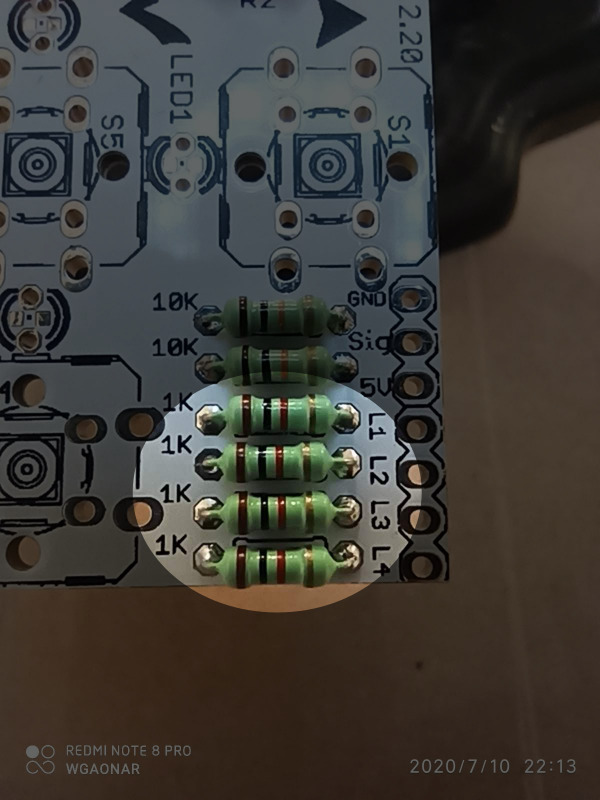
\includegraphics[width=0.9\columnwidth, height=1.2\columnwidth]{images/Botonera/botonera3.jpg}
        \caption{Resistencias R6, R8, R9, R10 de 1 K$\Omega$}
        \label{fig:botonera_resistencias3}
     \end{subfigure}
    \caption{Soldadura de las resistencias en la botonera parte 1.}
    \label{fig:botonera_resistencias_parte1}
\end{figure}

\begin{figure}[H]
    \ContinuedFloat \centering
    \begin{subfigure}[t]{0.3\textwidth}
        \centering
        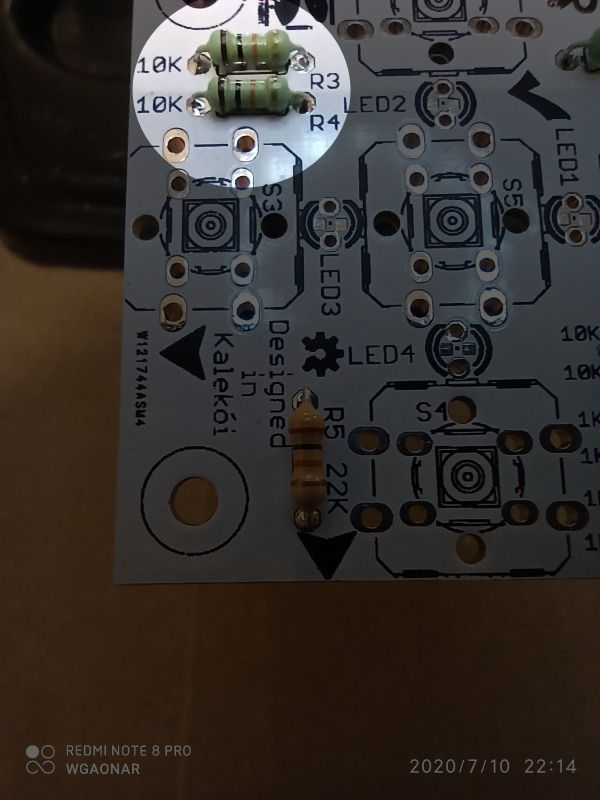
\includegraphics[width=0.9\columnwidth, height=1.2\columnwidth]{images/Botonera/botonera4.jpg}
        \caption{Resistencias R3, R4 de 10 K$\Omega$}
        \label{fig:botonera_resistencias4}
    \end{subfigure}%
    \begin{subfigure}[t]{0.3\textwidth}
        \centering
        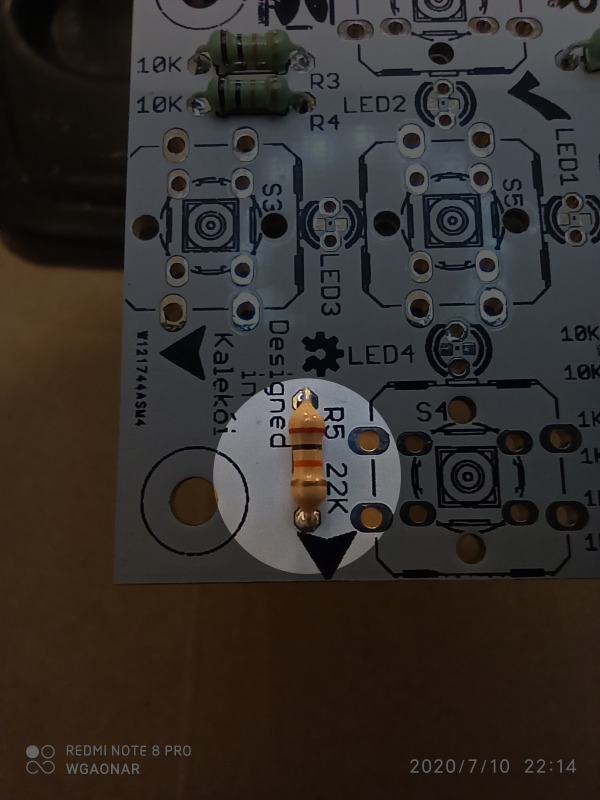
\includegraphics[width=0.9\columnwidth, height=1.2\columnwidth]{images/Botonera/botonera5.jpg}
        \caption{Resistencia R5 de 22 K$\Omega$}
        \label{fig:botonera_resistencias5}
    \end{subfigure}%
    \begin{subfigure}[t]{0.3\textwidth}
        \centering
        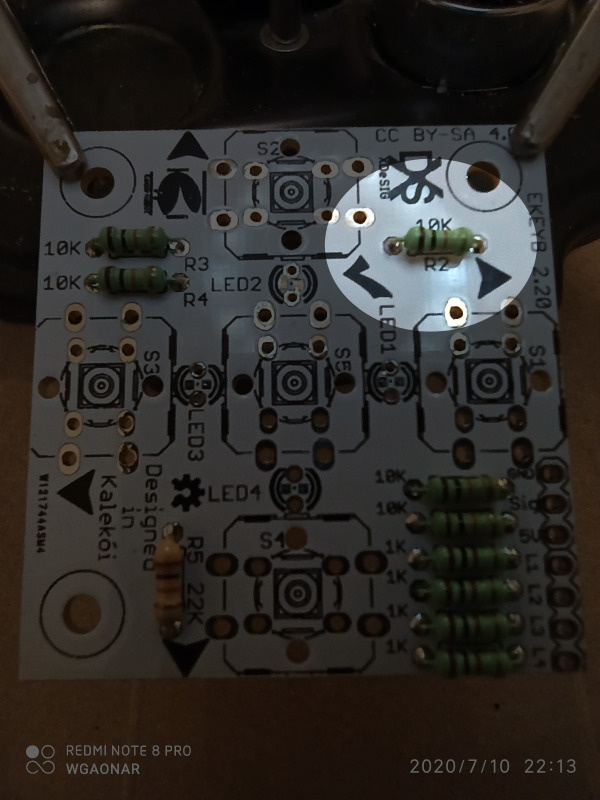
\includegraphics[width=0.9\columnwidth, height=1.2\columnwidth]{images/Botonera/botonera6.jpg}
        \caption{Resistencia R2 de 10 K$\Omega$}
        \label{fig:botonera_resistencias6}
    \end{subfigure}
    \caption{Soldadura de las resistencias en la botonera parte 2.}
    \label{fig:botonera_resistencias_parte2}
\end{figure}

\subsection{Soldadura de los Leds}
La lista de los Leds requeridos se muestra en la Tabla \ref{tab:componentes_botonera} en la que también se indica la posición de cada Led de acuerdo a su color y a su etiqueta en la tarjeta. Los Leds recomendados son de 3mm para que no estorben con los botones de 12mm. Antes de colocarlos en la tarjeta se tiene que fijar en la polaridad, ya que a diferencia de las resistencias, \textbf{\textcolor{red}{los Leds si tienen polaridad}}. Para ello, en la base cilíndrica del cuerpo de cristal del Led se puede observar una parte plana justo donde se conecta la terminal más corta que es la posición del cátodo o la terminal negativa del Led. 

\begin{figure}[H]
    \centering
    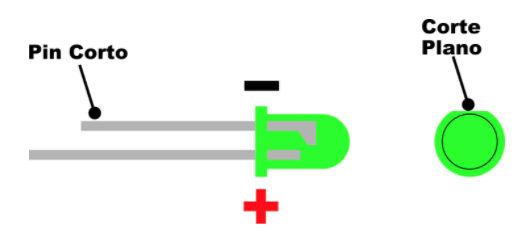
\includegraphics[width=0.5\columnwidth]{images/Botonera/led0}
    \caption{Esquema de polaridad del led.}
    \label{fig:poladirad_led}
\end{figure}

Si se observa la tarjeta de frente, el cátado de cada uno de los leds se orienta a la izquierda. Además, en el dibujo indicador de la tarjeta se puede observar, aunque muy sutilmente, esta parte plana. Soldar cada Led fijándose que la polaridad y el color coincida con la etiqueta en la tarjeta. Al finalizar de soldar todos los Leds, recortar los sobrantes. Los pasos en la soldadura de los Leds se puede observar en la Figura \ref{fig:botonera_leds}.

\begin{figure}[H]
    \centering
    \begin{subfigure}[t]{0.3\textwidth}
        \centering
        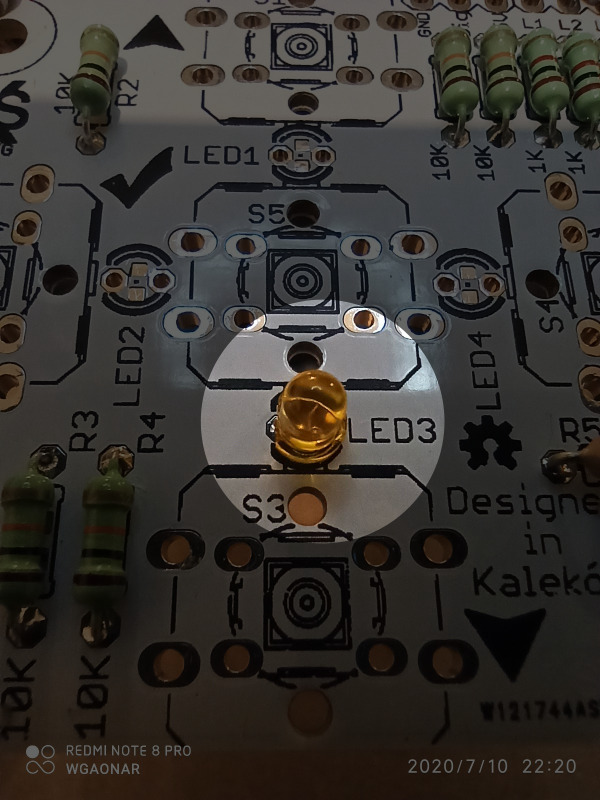
\includegraphics[width=0.9\columnwidth, height=1.2\columnwidth]{images/Botonera/led1.jpg}
        \caption{Led Amarillo (LED3).}
        \label{fig:botonera_led1}
    \end{subfigure}%
    \begin{subfigure}[t]{0.3\textwidth}
        \centering
        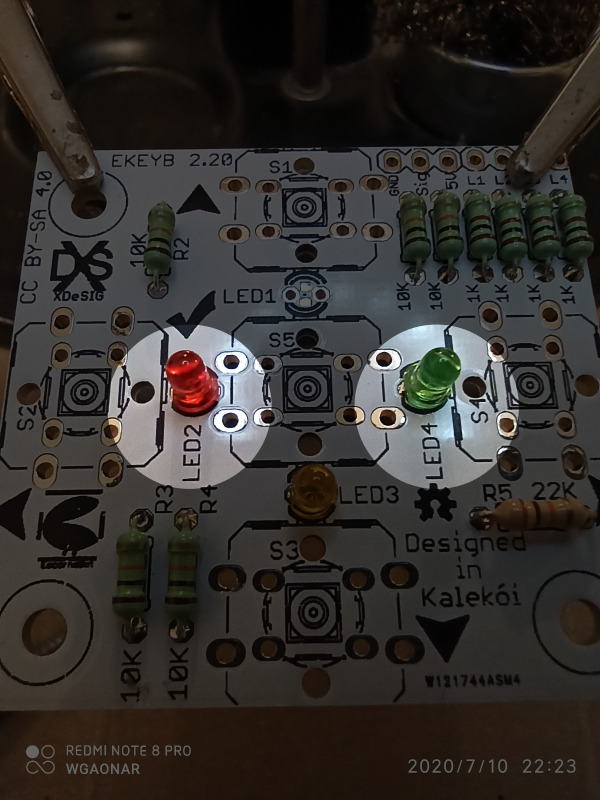
\includegraphics[width=0.9\columnwidth, height=1.2\columnwidth]{images/Botonera/led2.jpg}
        \caption{Leds Rojo (LED2 y Verde (LED4).}
        \label{fig:botonera_led2}
    \end{subfigure}
     
    \vspace{0.5cm}
    \begin{subfigure}[t]{0.3\textwidth}
        \centering
        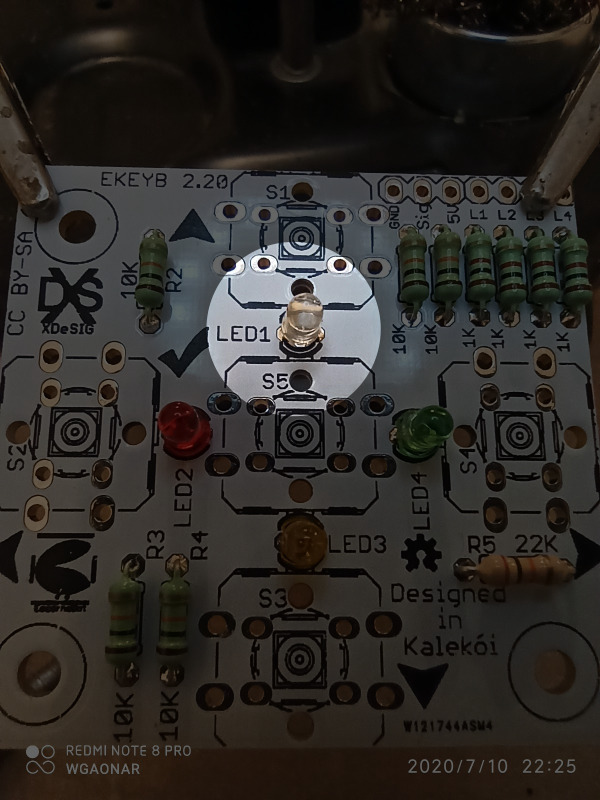
\includegraphics[width=0.9\columnwidth, height=1.2\columnwidth]{images/Botonera/led3.jpg}
        \caption{Led Azul (LED1), aunque en este caso el cuerpo es transparente, la luz que produce es color Azul}
        \label{fig:botonera_led3}
    \end{subfigure}%
    \begin{subfigure}[t]{0.3\textwidth}
        \centering
        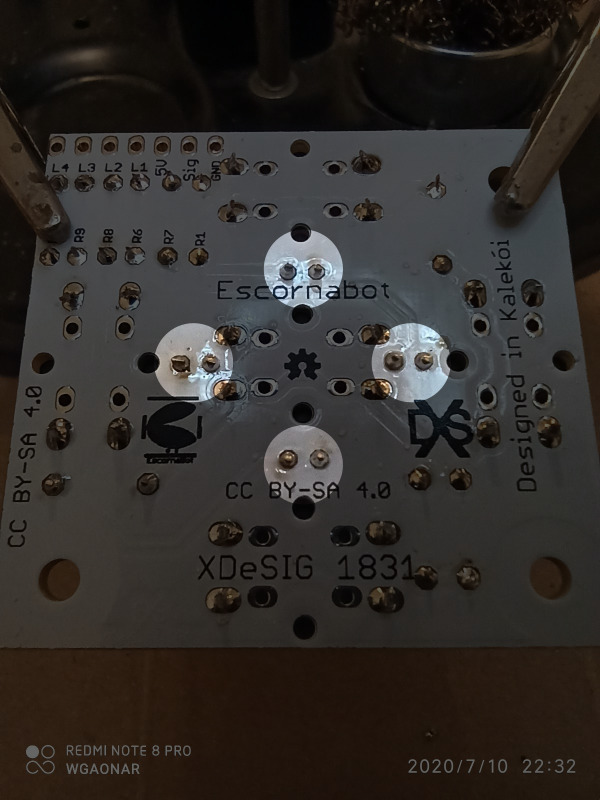
\includegraphics[width=0.9\columnwidth, height=1.2\columnwidth]{images/Botonera/led4.jpg}
        \caption{Terminales de los Leds recortadas.}
        \label{fig:botonera_led4}
    \end{subfigure}
    \caption{Soldadura de los leds en la botonera.}
    \label{fig:botonera_leds}
\end{figure}

\subsection{Soldadura de los Botones}
La soldadura de los botones se puede observar en la Figura \ref{fig:botones_soldadura}. Es simple de realizar ya que tienen las terminales dobladas formando un resorte para que se queden fijas en la tarjeta, basta insertarlos con cierta fuerza hasta que se escuche el sonido de un “click”, el cual indica que están fijos en su posición. 

\begin{figure}[H]
    \centering
    \begin{subfigure}[t]{0.3\textwidth}
        \centering
        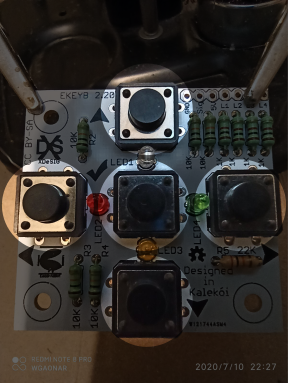
\includegraphics[width=0.9\columnwidth, height=1.2\columnwidth]{images/Botonera/botones1.png}
        \caption{Botones Soldados}
        \label{fig:botones_frente}
    \end{subfigure}%
    \begin{subfigure}[t]{0.3\textwidth}
        \centering
        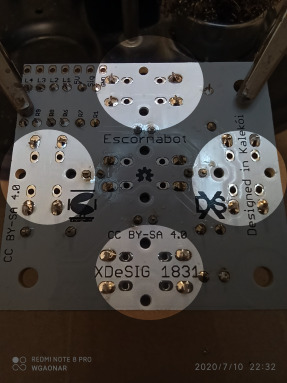
\includegraphics[width=0.9\columnwidth, height=1.2\columnwidth]{images/Botonera/botones2.jpg}
        \caption{Vista posterior con las terminales de los botones.}
        \label{fig:botones_posterior}
    \end{subfigure}
    \caption{Soldadura de los botones}
    \label{fig:botones_soldadura}
\end{figure}

\subsection{Soldadura de los Pines de Conexión}
La conexión con la placa EscornaCPU que contiene al Arduino Nano se realiza a través de 6 o 7 pines con las funciones listadas en la Tabla \ref{tab:pines_de_conexión}. La soldadura de los pines tipo macho a 90\degree se pueden ver en la Figura \ref{fig:pines_de_conexión}.

\begin{longtable}{|c|c|m{0.6\textwidth}|}
    \caption{Identificación de los pines de conexión \\ entre la botonera y la tarjeta EscornaCPU (Arduino Nano)} \label{tab:pines_de_conexión} \\ \hline 
    \multicolumn{1}{|c|}{\cellcolor[HTML]{C0C0C0}\textbf{PIN}} &
    \multicolumn{1}{|c|}{\cellcolor[HTML]{C0C0C0}\textbf{ETIQUETA}} & \multicolumn{1}{c|}{\cellcolor[HTML]{C0C0C0}\textbf{FUNCIÓN}} \\ \hline 
    \endfirsthead
    \caption{Identificación de los pines de conexión entre la botonera y la tarjeta EscornaCPU (Arduino Nano) - Continuación} \\ \hline
    \multicolumn{1}{|c|}{\cellcolor[HTML]{C0C0C0}\textbf{PIN}} &
    \multicolumn{1}{|c|}{\cellcolor[HTML]{C0C0C0}\textbf{ETIQUETA}} & \multicolumn{1}{c|}{\cellcolor[HTML]{C0C0C0}\textbf{FUNCIÓN}} \\ \hline 
    \endhead
    1 & GND & Trae la señal de tierra (0V) desde la tarjeta EscornaCPU (Arduino Nano). \\ \hline
    2 & Signal & Lleva la señal analógica del voltaje resultante al presionar uno de los botones. \\ \hline
    3 & 5V & \textcolor{red}{Opcional:} Está presente en la botonera en caso de que se utilice una tarjeta de control diferente a la EscornaCPU versión 1.2 y en la que no se utilice la resistencia interna de PULL-UP del Arduino Nano. En el firmware del robot se tendría que definir la palabra clave: KEYBOARD\_WIRES con valor de 3. \\ \hline
    4 & L1 & Señal de control para el Led 1 que indica un movimiento hacia ADELANTE. \\ \hline
    5 & L2 & Señal de control para el Led 2 que indica un movimiento hacia IZQUIERDA. \\ \hline
    6 & L3 & Señal de control para el Led 3 que indica un movimiento hacia ATRÁS. \\ \hline
    7 & L4 & Señal de control para el Led 4 que indica un movimiento hacia DERECHA. \\ \hline
\end{longtable}

\begin{figure}[H]
    \centering
    \begin{subfigure}[t]{0.3\textwidth}
        \centering
        \includegraphics[width=0.9\columnwidth, height=1.2\columnwidth]{images/Botonera/pinesdeConexión1.png}
        \caption{Pines de conexión vistos por detrás.}
        \label{fig:pines_de_conexión1}
    \end{subfigure}%
    \begin{subfigure}[t]{0.3\textwidth}
        \centering
        \includegraphics[width=0.9\columnwidth, height=1.2\columnwidth]{images/Botonera/pinesdeConexión2.png}
        \caption{Pines de conexión vistos de frente.}
        \label{fig:pines_de_conexión2}
    \end{subfigure}
    \caption{Soldadura de los pines de conexión en la botonera.}
    \label{fig:pines_de_conexión}
\end{figure}

\section{Ensamble y soldadura de la tarjeta de control EscornaCPU V1.2}
\subsection{Lista de componentes de la tarjeta de control}
\begin{longtable}{|c|>{\raggedright}m{0.15\textwidth}|>{\centering}m{0.15\textwidth}|m{0.5\textwidth}|}
    \caption{Descripción y funcionamiento de los componentes requeridos para la tarjeta de control} \label{tab:componentes_tarjeta_de_control} \\ \hline 
    \multicolumn{1}{|c|}{\cellcolor[HTML]{C0C0C0}\textbf{CANT.}} &
    \multicolumn{1}{c}{\cellcolor[HTML]{C0C0C0}\textbf{DESCRIPCIÓN}} & 
    \multicolumn{1}{|c|}{\cellcolor[HTML]{C0C0C0}\textbf{ETIQUETA}} & \multicolumn{1}{c|}{\cellcolor[HTML]{C0C0C0}\textbf{FUNCIÓN}} \\ \hline 
    \endfirsthead
    \caption{Componentes requeridos para la botonera - Continuación} \\ \hline
    \multicolumn{1}{|c|}{\cellcolor[HTML]{C0C0C0}\textbf{\makecell{CANT.}}} &
    \multicolumn{1}{c}{\cellcolor[HTML]{C0C0C0}\textbf{DESCRIPCIÓN}} & 
    \multicolumn{1}{|c|}{\cellcolor[HTML]{C0C0C0}\textbf{ETIQUETA}} & \multicolumn{1}{c|}{\cellcolor[HTML]{C0C0C0}\textbf{FUNCIÓN}} \\ \hline 
    \endhead
    1 & Arduino Nano & Arduino Nano & Tarjeta de desarrollo y programación basada en el microcontrolador ATmega328 \\ \hline
    1 & Driver ULN2803 & IC1 ULN2803 & Circuito integrado que es el enlace o interfaz entre las señales de control provenientes del Arduino Nano y los motores paso a paso 28BYJ-48. \newline \textbf{Nota:} \textcolor{red}{Este circuito no se solda}, se coloca sobre un zócalo o base que si irá soldado a la tarjeta. \\ \hline
    1 & Zócalo de 18 pines & IC1 ULN2803 & Base que soldada a la tarjeta sobre la que se coloca el driver ULN2803. \\ \hline
    1 & Terminal T-block & GND $+$ & Terminal de tornillos a los que se conectarán los cables provenientes del portapilas que alimentará la tarjeta de control y los motores paso a paso. \\ \hline
    \multirow{2}{*}{4} & \multirow{2}{4em}{Resistencia 10 K$\Omega$} & R1 & \textcolor{red}{Opcional:} Está presente en la tarjeta de control en caso de que se utilice una botonera diferente a la E\_KeyPad V2.2 que no cuente con esta resistencia y que no se utilice la resistencia interna de PULL\_UP del Arduino Nano. En el firmware del robot se tendría que definir la palabra clave: KEYBOARD\_WIRES con el valor de 3. Por precaución, esta resistencia se puede soldar. \\ \cline{3-4}
    &  & R2 & La primera resistencia del divisor de voltaje que reduce el voltaje de 5.0V a 3.3V que va desde el pin 1 del Arduino hacia el pin de transmisión del adaptador Bluetooth, en caso de que se desea conectar y utilizar. \\ \cline{3-4}
    &  & R4, R5 & \textcolor{red}{Opcionales:} Están presentes en la tarjeta de control en caso de que se desea conectar el Escornabot a una red WiFi a través de un módulo un ESP-01.  \\ \hline
    1 & Resistencia 18 K$\Omega$ o 20 K$\Omega$ & R3 & La segunda resistencia del divisor de voltaje que reduce el voltaje de 5.0V a 3.3V que va desde el pin 1 del Arduino hacia el pin de transmisión del adaptador Bluetooth, en caso de que se desea conectar y utilizar. \\ \hline
    \multirow{2}{*}{8} & \multirow{2}{0.15\textwidth}{Pines / headers macho rectos} & A0, A1, A2, A3, A7, GND & 6 Pines de conexión con la tarjeta de la botonera. \\ \cline{3-4}
    & & BUZZ ON & 2 Pines que permitirán activar / desactivar de forma manual el buzzer del Escornabot a través de la colocación de un puente o Jumper para pines rectos. \\ \hline
\end{longtable}

Seguir Escribiendo...

\end{document}
